\documentclass[9pt]{article}
\usepackage{a4wide}
\usepackage{graphicx}
\author{Martin Stransky}
\title{Tage data file description}

\begin{document}
\hyphenation{MODIFICATOR MASK}

\tableofcontents

\newpage
\section{Tage}

Tage is a texture and landscape generator focused to game developers. 
A scene is described by tage data files, some of them are 
in samples package.

\section{Tage datafile description}

This file describes tage input files format and grammar.

\section{Comments}

The input file uses standard C++ comments:
\begin{verbatim}
// One line comment

/*
  Two or more line comment
*/
\end{verbatim}

\section{Properties}

All properties are set by
\begin{verbatim}
property_name = value
\end{verbatim}
a "value" can be strings, numbers (hexa, integer, float-point), colors, vectors
and enumerated values.

\subsection{Boolean}

Boolean is a binary value (true/false) and it's used for switches
or on/off properties. The false value is written as 0 and true any other
number (typically 1).
\begin{verbatim}
// light is enabled 
enable_ligth = 1

// shadows are disabled
enable_shadows = 0
\end{verbatim}

\subsection{Numbers}

Numbers are standard numerical values and can have a decimal part.
\begin{verbatim}
size = 10
height = 1.1
\end{verbatim}

\subsection{Strings}

Strings don't use commas and can't contain spaces. String values are typically 
used for modificator/generator names.
\begin{verbatim}
name = my_modificator_name
\end{verbatim}

\subsection{Colors}
Colors can be defined by two ways - by separated RGB values (0-1) or (0-255),
by one hexadecimal digit (HTML color). There is an example
of color\_center set to R:33, G:25, B:7. The rgb() function converts
number from (0-255) range to (0-1) range.
\begin{verbatim}

// by RGB:
color_center.r = 0.12
color_center.g = 0.09
color_center.b = 0.02

// by RGB & rgb() function
color_center.r = rgb(33)
color_center.g = rgb(25)
color_center.b = rgb(7)

// by one hexa number (RRGGBB)
color_center = #211907

\end{verbatim}

The color type is stored internaly as tree float-point values and the 
.r .g and .b suffixes are normal numbers. You can use
common arithmetics operations like:

\begin{verbatim}

color_center.r = 0.12
color_center.g = color_center.r * 2
color_center.b = color_center.r / 4

\end{verbatim}

\subsection{Vectors}

Vectors are composed from two or three numbers. For instance, we want to 
set light\_position vector:
\begin{verbatim}
light_position.x = -1
light_position.y =  1
light_position.z = -1
\end{verbatim}
The .x,.y and .z suffixes are 0 by default. Another option is
to use a vector format (x,y,z):
\begin{verbatim}
light_position = (-1,1,-1)
\end{verbatim}

\subsection{Rectangles}

Rectangles defines a square area in a surface.
\begin{verbatim}
rect.x = 0
rect.y = 0
rect.dx = 20
rect.dy = 20
\end{verbatim}

\subsection{Angles}

An angles are normal numbers (an angle in degrees), from 0 to 360. 
They are used in polar coordinates and so on.
\begin{verbatim}
some_angle = 20.6
\end{verbatim}

\subsection{Enumerated types}

Enumerated types are values which can have some predefined values. 
They are typically used for blocks type descriptions, some types,
targets, operations and so on.
\begin{verbatim}
// coordinate type
type = MODIFICATOR_COORDINATE

// set modificator_target to texture
modificator_target = TEXTURE

// set modificator_target to geometry
modificator_target = GEOMETRY
\end{verbatim}

\subsubsection{Aritmetic operations}
It's one of frequently applied enumerated types and defines requested arithmetics
operation. It's used for coordinates, color/height operations and many more. Aritmetic 
operation anumerator is used in this context: 
\[
result = destination~OP~source
\]
where OP is defined as:

\begin{center}
  \begin{tabular}{|l||l|}
  \hline
  Operation & Meaning \\
  \hline
  \hline
  SET & \(result = source\) \\
  ADD & \(result = destination + source\) \\
  SUB & \(result = destination - source\) \\
  MODULATE & \(result = destination * source\) \\
  MODULATE2X & \(result = destination * source * 2\) \\
  \hline
  \end{tabular}
\end{center}

\subsection{Intervals}
Some values can be set as interval. If a value is an interval,
it means it can get any value from the border values. The border values
are marked as ".min" and ".max" suffixes. Intervals are always used
with other types (number, angle, color, vector). Intervals can be set 
as a normal (non-interval) value, too.
\begin{verbatim}
/* Number intervals
*/
// Interval set by only one value so it's always 10
angle = 10

// Interval set by two border values, 
// can be any value from 10 to 20
angle.min = 10
angle.max = 20 

/* Vector intervals
*/ 
// As components
position.min.x = 10
position.min.y = 10
position.min.z = 10

position.max.x = 20
position.max.y = 20
position.max.z = 20

// As vectors
position.min = (10,10,10)
position.max = (20,20,20)

/* Color intervals
*/
// As components
color.min.r = 10
color.min.g = 10
color.min.b = 10

color.max.r = 20
color.max.g = 20
color.max.b = 20

// As vectors
color.min = (10,10,10)
color.max = (20,20,20)

// As hexadecimal (HTML) colors
color.min = #0a0a0a
color.max = #141414
\end{verbatim}

\subsection{Coordinates}
Coordinates are 2D area which describes 
where a modificator is applied. The coordinate is a whole 
block with "type = MODIFICATOR\_COORDINATE", index (will be described later)
and start and size (or end) 2D vectors. There is an example of area
which starts at (0,0) and is 40x40 pixels wide:
\begin{verbatim}
{
  type = MODIFICATOR_COORDINATE

  index = 0

  start.x = 0
  start.y = 0

  size.x = 40
  size.y = 40
}
\end{verbatim}

\section{Basic blocks}
An atomic part of the file is a block inside compound braces. It describes one 
atomic unit inside generator or some generator values. Each block must
contain its name and type.
\begin{verbatim}
{
  name = generator
  type = GENERATOR_MESH

  /* All generator params come here
  */
}
\end{verbatim}
Blocks can be nested, like this one:
\begin{verbatim}
/* Describes pixel generator and its color definition
*/
{
  name = pixel_point
  type = MODIFICATOR_POINT_SINGLE

  {
    type = MODIFICATOR_POINT_SINGLE_COLOR
    color_center = #3b5528
  }
}
\end{verbatim}
All block examples bellow uses this format:
\begin{verbatim}
{
  /* First part contains block name and type:
  */
  name = block_name
  type = block_type

  /*
    Second part is a list of all posible properties,
    descriptions and default values:

    [property_type]  property_name
   
    If the property_type is an enumerated type, all 
    posibilies come here:
    
    VALUE_1
    VALUE_2
    VALUE_3
  */  
  property_name = default_value_of_the_property
}
\end{verbatim}

\newpage
\section{Tage generator architecture}
Whole generator is designed as a modificator chain. There is one master (root)
modificator and it passes results to slave modificators. A last modificator 
in the chain writes results (color pixel, heights) directly to a generator target
(it can be mesh itself, mesh texture or something else).

\begin{figure}[h]
\begin{center}
  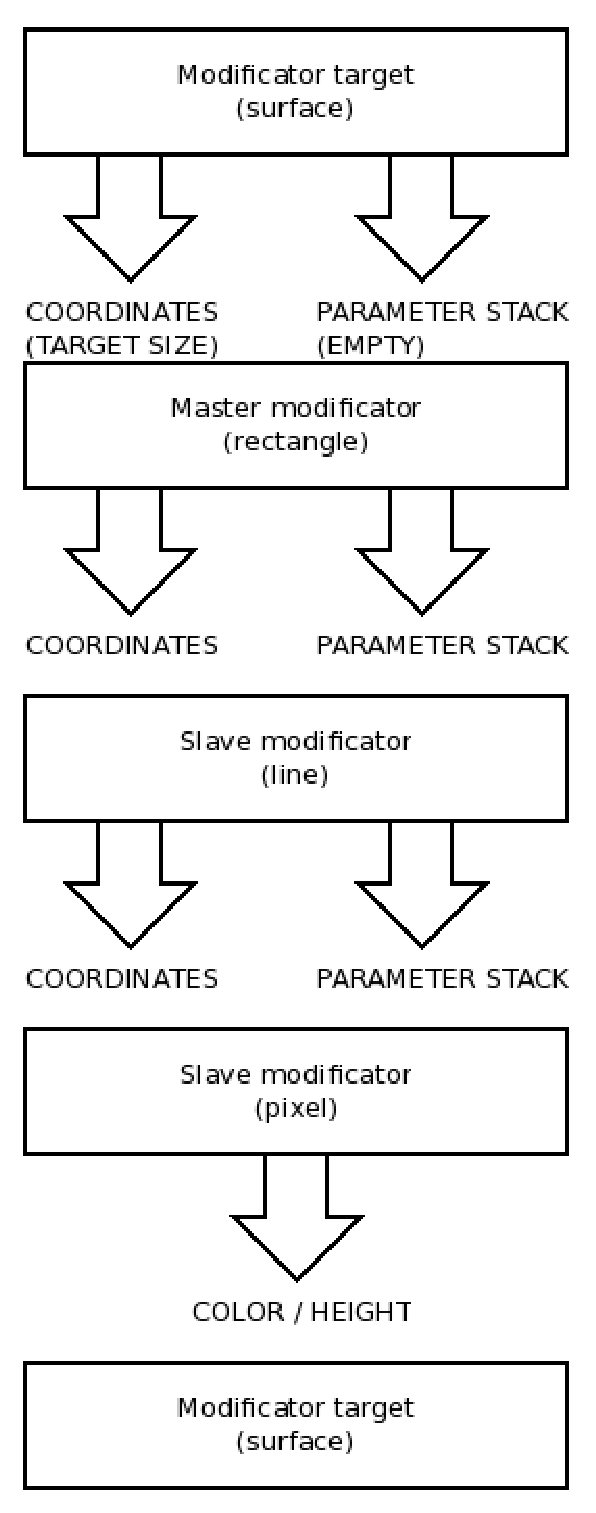
\includegraphics[scale=0.6]{p08.eps}
  \caption{Modificator chain which draws a line composed from single pixels.}
  \label{rect_line_example}
\end{center}
\end{figure}

A picture \ref{rect_line_example} is a nice example of a modificator chain. The first
modificator here is the rectangle and it's applied to whole
target surface because local coordinates are not defined. If the target surface
is 2048 pixels wide and 1024 pixels high, the rectangle will get \begin{math}(0,0) 
-> (2048, 1024)\end{math} coordinates. 

By default the rectangle modificator paints whole area by pixels. So it calls
specified slave modificator (the line here) for each pixel inside the \begin{math}(0,0) 
-> (2048, 1024)\end{math} target surface area.

A next modificator here is the line and it's drawn for each pixel inside the
target surface. We can define (by coordinate block inside the line modificator) the line
size and direction so we can obtain a rectangle filled by single lines. 
The lines are composed from single pixels which are drawn by 
the last modificator here - pixel.

\begin{itemize}
\item{\bf Modificators} are atomic generator parts specialized to one task. 
Each modificator is configured by properties (from the data file), 
coordinates (from the data file and/or previous modificator) and 
parameters (from previous modificator) and pastes its results 
(coordinates, properties, parameters) to another modificator.

For instance there is a modificator which generates a line and it 
pastes the results (coordinates for each single point which lies on the line) 
to another modificator which draws them. A final modificator writes single
pixels to generator target which stands for final texture or a flat mesh.

\item{\bf Targets} are "final" modificators which can transform
results (color, height) into geometry (mesh) or texture. Each 
target has defined size (like texture size, mesh size and so on).

A special type of target is an auxiliary target 
(it's a kind of color and height cache), generator target 
(launches defined generator with specified coordinates) and modificator target
(writes color or height to mask or heightmap modificator).

\item{\bf Generator} joins modificators and targets to one object with name. 
One modificator or target can be used by multiple generators.

Generator itself can be used as a modificator so
if we take the line modificator from previous example:
\[
line~modificator~->~pixel~modificator~->~texture~target
\]
will generate single pixels to texture, but this one:
\[
line~modificator~->~pixel~modificator~->generator~target
\]
can generate 3D objects on given coordinates (for instance when you want to
generate grass bunches on square area).

\item{\bf Generator launcher} can launch any generator which was defined.

\end{itemize}

\newpage
\section{Generator launcher}
Generator launcher defines which generators are performed and their order. 
It can be only one in the whole data file.
\begin{verbatim}
{
  /* Launcher name and type
  */
  name = generator_launcher_name
  type = GENERATOR_LAUNCHER

  /* Performed generators. 
  */
  generator_mesh = first_generator
  generator_mesh = second_generator
  generator_mesh = third_generator
}
\end{verbatim}

\newpage
\section{Generator}

Generator defines which modifiators are launched, their targets and order.
There can be as many generators as you want in a data file.

\begin{verbatim}
/* A simple generator
*/
{
  /* Generator name and type
  */
  name = generator_name
  type = GENERATOR_MESH

  /*
    Modificator name and its target:
    
    [string]          modificator
    [enumerated type] modificator_target
      
      TEXTURE
      GEOMETRY
      GENERATOR_MESH
      AUX
      MODIFICATOR
      
    [string]          modificator_target_name
  */
  
  /*
    Mask properties:
    
    [...]  
  */
}
\end{verbatim}
\subsubsection*{Generator items}
\begin{itemize}
\item{\bf modificator} - launches a modificator with this name and all his child modificators.
\item{\bf modificator\_target} - defines a target for this modificator and his child modificators.
\begin{itemize}
\item{\bf TEXTURE} - a final texture of generated object. The target also contains height pixels
but they are not used in the final texture, but the height data can be read and used for shading.
\item{\bf GEOMETRY} - final heights in generated mesh geometry. Color data written to this target
is transformed to height (as intensity of light).
\item{\bf GENERATOR\_MESH} - target is another generator.
\item{\bf AUX} - an auxiliary surface (color and height). Generated data from {\bf AUX} target 
can be read by MODIFICATOR\_TARGET modificator and processed to another target, like the final texture or mesh. 
You have to specify {\bf modificator\_target\_name} of the {\bf AUX} target.
\item{\bf MODIFICATOR} - target is a modificator defined with {\bf modificator\_target\_name}. 
Supported target modifiators can be MODIFICATOR\_MASK and 
MODIFICATOR\_HEIGHT\_MAP for now.
\end{itemize}
\item{\bf modificator\_target\_name} - name of target modificator. It's useful
when referenced modificator can have more than one instance. If the name is unset,
a first target of defined type is choosen.
\end{itemize}

\subsubsection*{Mask properties}
Each target can have attached a mask which is applied to all pixels (color/height) 
written to the target. The properties are described in section \ref{mask_properties}. 

\subsubsection*{There is an example of a simple generator there:}

\begin{verbatim}
/* A simple generator
*/
{
  /* Generator name and type
  */
  name = generator_name
  type = GENERATOR_MESH
  
  /* First modificator chain writes to texture
  */
  modificator = first_modificator
  modificator_target = TEXTURE
  
  /* Second modificator chain writes to mesh
  */
  modificator = modificator_name  
  modificator_target = GEOMETRY
}
\end{verbatim}

\subsection{Multiple generator targets}
\label{multiple_targets}

Look at this example:

\begin{verbatim}
/* A simple generator
*/
{
  /* Generator name and type
  */
  name = generator_name
  type = GENERATOR_MESH
  
  /* A modificator chain writes to mesh and texture
  */
  modificator = modificator_name
  modificator_target = TEXTURE
  modificator_target = GEOMETRY
}
\end{verbatim}

As you can see you may define more (up to five) targets for each modificator. 
If the targets have different sizes (e.g. texture is 512x512 pixels wide 
and generated mesh is a landscape with 20x20 points), the second and further 
targets are scaled according the first one (i.e. the geometry here will have 
512x512 temporary points and they will be scaled to the final 20x20 grid).

\newpage
\section{Generator targets}
A 3D objects generated by a single generator is usually a flat mesh with
one big texture. If the texture is too big, it's sliced to smaller parts.
The object is described by mesh, material and texture block.

\subsection{Geometry target}

The geometry target is defined by one MESH\_PARAMS block. It defines 
mesh properties like type, size and so on. If it's missing in the 
tage file, default values are used for the generated mesh.

\begin{verbatim}
{
  name = mesh_name
  type = MESH_PARAMS

  /*
    [enumerated value]  mesh_type
   
      MESH_LAND
      MESH_BUNCH
      MESH_GRASS
      MESH_BUSH
  */
  mesh_type = MESH_LAND
  
  /*
    Mesh dimensions. All values are vector intervals.
  
    [vector, interval] start
    [vector, interval] diff
    [vector, interval] size
  */  
  start = (0,0,0)
  diff = (1,1,1)
  size = (1,1,1)
  
  /*
    Parameters related to bunch:
    
    [int, interval]   bunch_slice_num
    [int, interval]   bunch_slice_segments
      
    [float, interval] bunch_slice_x_offset
    [float, interval] bunch_slice_z_offset

    [float, interval] bunch_slice_width_start
    [float, interval] bunch_slice_width_end
    
    [float, interval] bunch_slice_height_start
    [float, interval] bunch_slice_height_end

    [angle, interval] bunch_slice_falling
    [angle, interval] bunch_segment_falling
        
    [int]             bunch_slice_rotation_incemental
    [angle, interval] bunch_slice_rotation_range
    [angle, interval] bunch_slice_rotation_step
  */    
  bunch_slice_num = 6
  bunch_slice_segments = 1
  
  bunch_slice_x_offset = 0
  bunch_slice_z_offset = 0
  
  bunch_slice_width_start = 1
  bunch_slice_width_end = 1
  
  bunch_slice_height_start = 1
  bunch_slice_height_end = 1
  
  bunch_slice_falling = 0
  bunch_segment_falling = 0
  
  bunch_slice_rotation_incemental = 0
  bunch_slice_rotation_range = 180
  bunch_slice_rotation_step = 0
}
\end{verbatim}
\subsubsection*{Mesh items}
\begin{itemize}
\item{\bf mesh\_type} - defines a type of generated object. 
\begin{itemize}
\item{\bf MESH\_LAND} - a flat land
\item{\bf MESH\_BUNCH} - a bunch of plates
\item{\bf MESH\_GRASS} - not implemented yet
\item{\bf MESH\_BUSH} - not implemented yet
\end{itemize}

Land:

\item{\bf start} - mesh location
\item{\bf diff} - a size of one segment
\item{\bf size} - number of segments

Bunch:

\item{\bf start} - bunch location
\item{\bf diff} - a size of one bunch slice
\item{\bf size} - unused (number of segments in one slice is controlled by {\bf bunch\_slice\_segments}

\item{\bf bunch\_slice\_num}
\item{\bf bunch\_slice\_segments}

\item{\bf bunch\_slice\_x\_offset}
\item{\bf bunch\_slice\_z\_offset}

\item{\bf bunch_slice_width_start}
\item{\bf bunch_slice_width_end}

\item{\bf bunch_slice_height_start}
\item{\bf bunch_slice_height_end}

\item{\bf bunch\_slice\_falling}
\item{\bf bunch\_segment\_falling}

\item{\bf bunch\_slice\_rotation\_incemental}
\item{\bf bunch\_slice\_rotation\_range}
\item{\bf bunch\_slice\_rotation\_step}
\end{itemize}

\newpage
\subsection{Texture target}

The texture target is defined by two blocks - TEXTURE\_PARAMS and MATERIAL\_PARAMS.

\subsubsection*{Texture parameters}

This block representes a texture of generated object. If it's missing in the 
tage file, default values are used for the generated texture.

\begin{verbatim}
{
  name = test_texture
  type = TEXTURE_PARAMS

  /*
    [vector]  texture_size
    [int]     texture_height
    [color]   background_color
    [int]     texture_alpha
  */
  texture_size = (512,512)
  texture_height = 512
  background_color = #000000
  texture_alpha = 0
}
\end{verbatim}
\subsubsection*{Texture items}
\begin{itemize}
\item{\bf texture\_size} - size of generated texture, it's limited only by available system memory.
\item{\bf texture\_height} - imaginary texture height, has effect for shading (light).
\item{\bf background\_color} - default texture color.
\item{\bf texture\_alpha} - use alpha component for the texture.
\end{itemize}

\subsubsection*{Material parameters}

You can modify some texture parameters of generated mesh. If it's missing in the 
tage file, default values are used for the generated texture.

\begin{verbatim}
{
  name = test_material
  type = MATERIAL_PARAMS
  
  /*
    [boolean] transparent
    [boolean] double_side
  */
  transparent = 0
  double_side = 0  
}
\end{verbatim}
\subsection*{Material items}
\begin{itemize}
\item{\bf transparent} - the generated texture is transparent.
\item{\bf double\_side} - double sided material, it's used by bunches, grass and so.
\end{itemize}

\newpage
\subsection{Auxiliary target}

Describes a helper target which contains color and height components. 
The parameters are identical with the texture ones. If you want to use color 
or height pixels written to this target you need to use a MODIFICATOR\_TARGET
modificator.

\begin{verbatim}
{
  name = aux_target
  type = AUX_PARAMETERS

  /*
    [vector]  aux_size
    [int]     aux_height
    [color]   background_color
    [int]     aux_alpha
  */
  aux_size = (512,512)  
  aux_height = 512
  background_color = #000000
  aux_alpha = 0
}
\end{verbatim}
\subsubsection*{Texture items}
\begin{itemize}
\item{\bf aux\_size}
\item{\bf aux\_height}
\item{\bf background\_color}
\item{\bf aux\_alpha}
\end{itemize}

\subsection{Generator mesh target}
GENERATOR\_MESH
TODO

\newpage
\section{Generator modificators}

\subsection{A generic modificator blocks}

There are some properties which can be included in 
any modificator block, but not all properties are 
available in all modificators and some 
can have a different meaning.

\subsubsection{Pixel properties}

Pixel properties control pixel generation. 

\begin{verbatim}
  /*
    [boolean] area_inverted
    
    [int]     pixel_size
    
    [int]     pixel_step
    [int]     pixel_step_x
    [int]     pixel_step_y
  
    [boolean] pixel_step_random
    [int]     pixel_step_random_min
    [int]     pixel_step_random_max
    
    [float]   pixel_color_density
    
    [boolean] probability_fade
    [float]   probability_fade_start
    [float]   probability_fade_stop
  
    [boolean] color_fade
    [float]   color_fade_start
    [float]   color_fade_stop
      
    [boolean] erode_border
    [float]   erode_factor
  */    
\end{verbatim}

\begin{itemize}
\item{\bf area\_inverted} - inverted rendering.
\item{\bf pixel\_size} - size of single pixel. It's used only by MODIFICATOR\_POINT\_SINGLE.
\item{\bf pixel\_step} - distance between pixels, draws grid instead of solid surface.
\item{\bf pixel\_step\_x} - distance between pixels in X asis.
\item{\bf pixel\_step\_y} - distance between pixels in Y asis.
\item{\bf pixel\_step\_random} - randomize pixel distances.
\item{\bf pixel\_step\_random\_min, pixel\_step\_random\_max} - pixel distance boundary. 
\item{\bf pixel\_color\_density} - a probability of pixel emission, from
\begin{math}<0,1>\end{math} range.
\item{\bf probability\_fade} - pixel probability fading, it's used by MODIFICATOR\_POINT\_EXTENDED only.
\item{\bf probability\_fade\_start}
\item{\bf probability\_fade\_stop}
\item{\bf color\_fade} - pixel color fading, it's used by MODIFICATOR\_POINT\_EXTENDED only.
\item{\bf color\_fade\_start}
\item{\bf color\_fade\_stop}
\item{\bf erode\_border} - pixel border erosion.
\item{\bf erode\_factor}
\end{itemize}

\subsubsection{Mask properties}
\label{mask_properties}

Every modificator can use a mask. The mask controls if and how are
modificator pixels (color/height) passed to slave modificator(s). The mask itself 
has to be defined as MODIFICATOR\_MASK modificator first and then referenced
from this modifiator. Mask is controlled by those properties:

\begin{verbatim}
  /*
    [string]              mask
    
    [aritmetic operation] mask_op
    [boolean]             mask_blend
    [boolean]             mask_dithering
    
    [boolean]             mask_create
    [boolean]             mask_inverted
    [integer]             mask_overlapping
    
    [color]               mask_color
    [float]               mask_height
    [float]               mask_height_min
    [float]               mask_height_max
  */
\end{verbatim}

\begin{itemize}
\item{\bf mask} - a name of a mask modificator (defined as MODIFICATOR\_MASK class).
\item{\bf mask\_op} - an operation between source and target pixels (color/height). 
It's used when modificator writes directly to some target (a texture for instance).
\item{\bf mask\_blend} - allow/disable blending (for fuzzy mask borders).
\item{\bf mask\_dithering} - allow/disable dithering (for fuzzy mask borders).
\item{\bf mask\_create} - if you set this option, the target mask modificator will be created
when this modificator tries to operate with the mask for first time. It's used when one 
modificator draws to the mask and another one reads the data.
\item{\bf mask\_inverted} - inverted mask application.
\item{\bf mask\_overlapping} - enables fuzzy mask borders, defines how big the fuzzy
borders are.
\item{\bf mask\_color} - if target mask is MASK\_COLOR type, defines which color
is considered as "true" value.
\item{\bf mask\_height} - if target mask is MASK\_HEIGHT type, defines which color
is considered as "true" value.
\item{\bf mask\_height\_min, mask\_height\_max} - if target mask is MASK\_HEIGHT type,
defines a corner values for fuzzy border. {\bf mask\_height\_min} means no mask application
and {\bf mask\_height\_max} means full mask application.
\end{itemize}

\subsubsection{Mask creation}

A content of MODIFICATOR\_MASK (the mask) can be created when 
the modificator is called for first time. Mask type and other mask configuration
is set in MODIFICATOR\_MASK block besides the mask size which is a size 
of area where the modificator is applied. There are two types of created mask:

\begin{verbatim}
  /*
    [string]              mask_create
    [string]              mask_create_remove
  */
\end{verbatim}

\begin{itemize}
\item{\bf mask\_create} - mask referenced by this option is created before 
the modificator execution. If the mask already exists, the directive is ignored and
mask is not modified.
\item{\bf mask\_create\_remove} - mask referenced by this option is created before 
modificator execution and it's removed when modificator finishes.
\end{itemize}

\subsubsection{Slave modificators}

Almost every modificator (except the MODIFICATOR\_POINT\_SINGLE) needs to 
have defined a slave modificator. You can define up to five slave modificators 
for each class (slave, pre, post) and those modificators are called in 
order how they are defined.

\begin{verbatim}
  /*
    [string] modificator_slave
    [string] modificator_pre
    [string] modificator_post
  */  
\end{verbatim}

\begin{itemize}
\item{\bf modificator\_slave} - is called for each pixel generated 
by this modificator.
\item{\bf modificator\_pre} - is called before this modificator starts 
and with top coordinates only.
\item{\bf modificator\_post} - is called when the modificator finishes 
and with top coordinates only.
\end{itemize}

So imagine there's a MODIFICATOR\_RECT which generates a rectangle area 
from \((20,20)\) to \((50,50)\). It means that:

\begin{itemize}
\item{\bf modificator\_pre} is called before the pixels are emitted with 
coordinates \newline\(x = 20~y = 20~width = 30~height = 30\).
\item{\bf modificator\_slave} is called for each pixel
from \((20,20)\) to \((50,50)\) with \newline\(width = 1~height = 1\).
\item{\bf modificator\_post} is called when all pixels are emitted
with coordinates \newline\(x = 20~y = 20~width = 30~height = 30\).
\end{itemize}

\subsubsection{Local coordinates setup}

Each modificator can contain local coordinate setup. It's defined by nested 
MODIFICATOR\_COORDINATE block and other properties described in next chaper.

\newpage
\subsection{Coordinates}
Each modificator is applied to an area which is restricted by "top" coordinates. 
Top coortinates are defined by master modificator or size of target surface 
for the first modificator.

\begin{figure}[h]
\begin{center}
  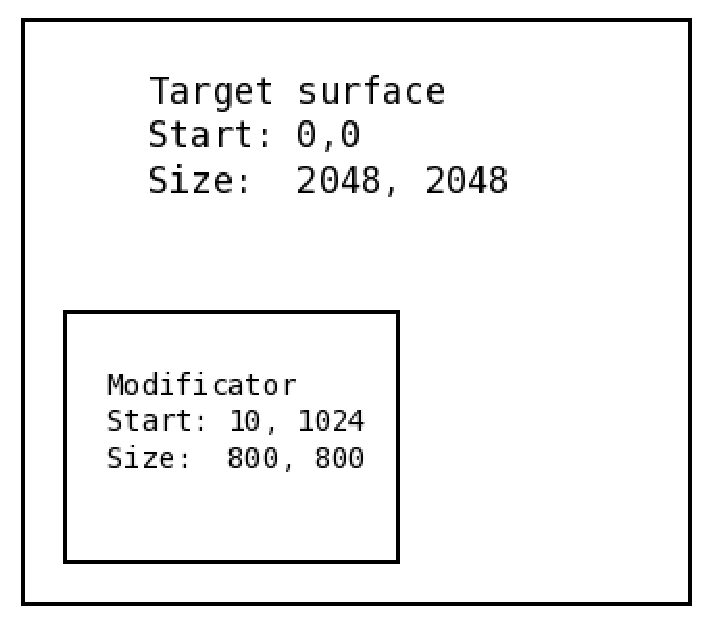
\includegraphics[scale=0.6]{p02.eps}
  \caption{Target surface and one modificator.}
\end{center}
\end{figure}

Those "top" coordinates are further modified by local
coordinate block (randomization, size extension
and so on).

\subsubsection{Coordinate block}
Defines a block with {\bf local} coordinate configuration. 
Top coordinates are defined by master modificator or modificator target and
local coordinates are defined by coordinate block which can be included in
any modificator.

\begin{figure}[h]
\begin{center}
  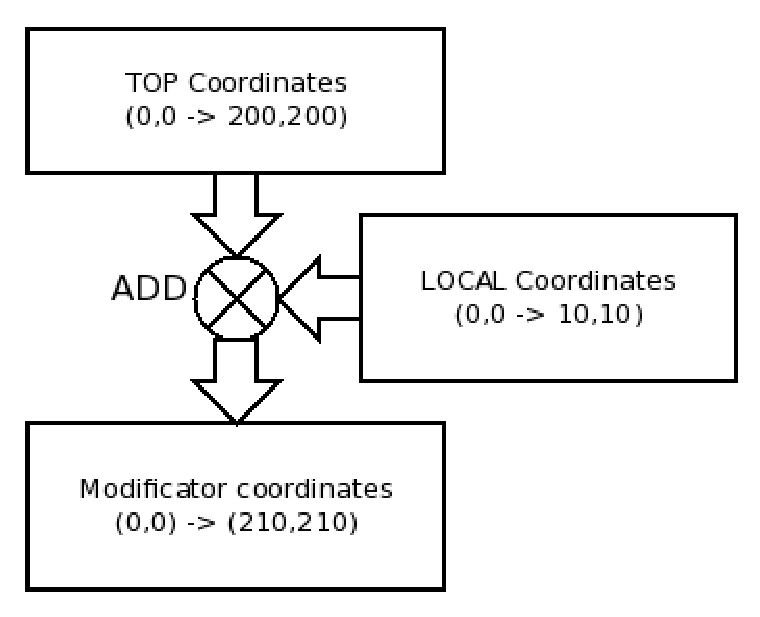
\includegraphics[scale=0.6]{p06.eps}
  \caption{An example of top and local coordinates composition.}
\end{center}
\end{figure}

Coordinate properties define operations between top and local coordinates, 
whether the local ones are generated (randomized) or not and so forth. 
If there are more than one MODIFICATOR\_COORDINATE block, 
the modificator is called for each of them 
(see figure \ref{coord_modificator_chain}).

\subsubsection*{Coordinate setup properties}
\begin{verbatim}
  /*
    Local coordinates setup:
    
    [aritmetic operation] coordinates_operation 
    [boolean]             coordinates_random
    [int]                 coordinates_random_num
    [enumerated type]     modificator_start
    [enumerated type]     modificator_size
            
      COORD_CURRENT
      COORD_LAST_START
      COORD_LAST_SIZE
      COORD_LAST_START_SIZE      
  */  
  coordinates_operation = OPERATION_SET
  coordinates_random = 0
  coordinates_random_num = 0
  modificator_start = COORD_CURRENT
  modificator_size = COORD_CURRENT
  
  /*
    First coordinates blocks:
  */
  {
    type = MODIFICATOR_COORDINATE
    
    /*
      [vector] start
      [vector] size
      [int]    index
    */
  }
  
  /*
    Second coordinates blocks:
  */
  {
    type = MODIFICATOR_COORDINATE
    
    /*
      [vector] start
      [vector] size
      [int]    index
    */
  }
  
  /*
    Third one...
  */
  {
    [...]
  }
\end{verbatim}
\subsubsection*{Coordinate block properties}
\begin{itemize}
\item{\bf coordinates\_operation} - defines operation between top and local coordinates.
\item{\bf coordinates\_random} - if it's set to 1, local coordinates are generated by random number
generator in boundaries given by coordinates with index 0 and index 1 (see bellow).
\item{\bf coordinates\_random\_num} - number of generated local coordinates.    
\item{\bf modificator\_start, modificator\_size} - it defines parts of top 
coordinates (start and size parts) for current coordinates\_operation. 
It can be top coordinates from previous modificator (COORD\_CURRENT) or 
result of last top and local coordinates composition:
\begin{itemize}
\item{\bf COORD\_CURRENT} - current top coordinates
\item{\bf COORD\_LAST\_START} - start of last coordinate composition (start part)
\item{\bf COORD\_LAST\_SIZE} - size of last coordinate composition (size part)
\item{\bf COORD\_LAST\_START\_SIZE} - endpoint of last coordinate composition (start+size parts).
It's userful for generating objects which have to be connected (e.g. objects strips).
\end{itemize}
\end{itemize}
\subsubsection*{Modificator coordinate sub-block properties}
\begin{itemize}
\item{\bf start} - coordinate start
\item{\bf size} - coordinate size, endpoint is calculated as start+size
\item{\bf index} - coordinate index (used by randomized local coordinates, see bellow)
\end{itemize}

\begin{figure}[h]
\begin{center}
  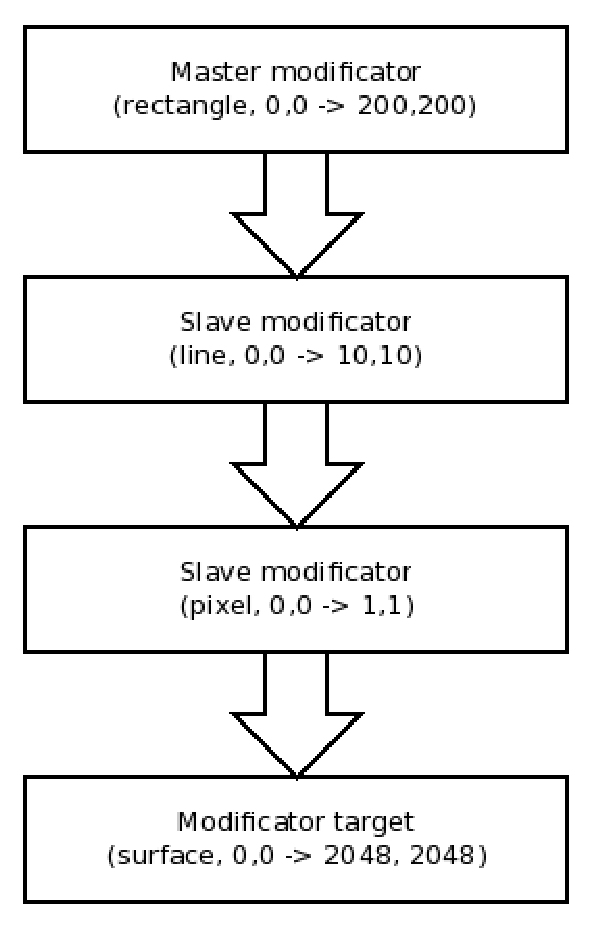
\includegraphics[scale=0.6]{p05.eps}
  \caption{An example of modificator chain with local coordinate setup.}
  \label{coord_modificator_chain}
\end{center}
\end{figure}

\newpage
\subsection{Modificator parameters}

Parameters are float point values in \begin{math}<0,1>\end{math} range which are passed between
modificators on parameter stack. If a modificator generates any parameter, the
parameter is added on top of the parameter stack. If a modificator does not
emit any parameter the stack is passed without modification.

The parameters and are typically used by simple point modificator 
for color/height generation and so on. For instance, there's a fractal
modificator which generates a height map. The fractal modificator calls
a slave modificator (simple point modificator for instance) for each generated 
pixel and as parameter passes pixel height. So the slave pixel modificator can 
draw pixels by color adjusted by pixel height. Another example showns 
figure \ref{rect_line_example}.

There is a list of available modificator parameters:

\begin{center}
  \begin{tabular}{|l||p{10cm}|}
  \hline
  PARAM\_PREV\_0 & a parameter on top of the parameter stack \\
  PARAM\_PREV\_1 & a second one \\
  PARAM\_PREV\_2 & third one \\
  ... & \\
  PARAM\_PREV\_9 & \\
  PARAM\_RAND & a random number from \begin{math}<-1,1>\end{math} with normal distribution \\
  PARAM\_RAND\_HALF & a random number from \begin{math}<0,1>\end{math} with normal distribution \\
  PARAM\_GAUSS & a random number from \begin{math}<-1,1>\end{math} with gaussian distribution \\
  PARAM\_GAUSS\_HALF & a random number from \begin{math}<0,1>\end{math} with gaussian distribution (center is in 0) \\
  \hline
  \end{tabular}
\end{center}

\newpage
\subsection{Point modificators}

Point modificators are designed as last modificators and usually write
data directly to targets (height to mesh geometry or color/heights to texture). 

\subsubsection{Single point modificator}

Single point modificator writes to target (slave modificator
or texture target) only one single point. Its size is always 1x1 so for instance
if it gets \begin{math}(20,20) -> (100,100)\end{math} coordinate 
from master modificator, it writes only single pixel to \begin{math}(20,20)\end{math} 
with \begin{math}(1,1)\end{math} size. Pixel\_size property is ignored 
by this modificator.

The single point modificator consists from basic setup in main block and
subblocks. A subblock defines particular color/height operations applied to 
any pixel processed by single point modificator. Number of color/height 
subblocks is not limited.

There are two types of subblocks. MODIFICATOR\_POINT\_OPBOX is applied to 
each pixel which is processed by the single point modificator. For instance when 
a parent modificator is a MODIFICATOR\_RECT then the MODIFICATOR\_POINT\_OPBOX
is applied to all pixels inside the generated rectangle.

On the other hand the MODIFICATOR\_POINT\_OPBOX\_INIT block (which is a sub block of 
MODIFICATOR\_POINT\_OPBOX is called only once when the parent modificator
starts to emit the pixels by MODIFICATOR\_POINT\_OPBOX. So it allows to set 
values which are constant in all calls of MODIFICATOR\_POINT\_OPBOX.

\subsubsection*{Single point modificator block contains}
\begin{verbatim}
{
  name = some_modificator_name
  type = MODIFICATOR_POINT_SINGLE
  
  /*
    Generated colors can be crop:
  
    [boolean]               color_borders
    [color]                 color_border_min
    [color]                 color_border_max
   */
  color_borders = 0
  color_border_min = (0,0,0)
  color_border_max = (255,255,255)
  
  /*
    Color tables:
          
    [string]                color_table
  */
  
  /*
    A subblock
  */
  {
    type = MODIFICATOR_POINT_OPBOX
    
    /*
      Write color/height to target pixels
    */
    
    [...]
    
    {
      type = MODIFICATOR_POINT_OPBOX_INIT
      
      /*
        Initialize values for parent 
        MODIFICATOR_POINT_OPBOX block
      */
            
      [...]
    }
  }
  
  /*
    Another subblock
  */
  {
    type = MODIFICATOR_POINT_OPBOX
    [...]
  }
}
\end{verbatim}
\subsubsection*{Single point modificator properties}

\begin{itemize}
\item{\bf color\_borders} - are generated colors shrink to this range?
\item{\bf color\_border\_min} - minimal border color
\item{\bf color\_border\_max} - maximal border color
\end{itemize}
Color table can define a colors which can be used for color generation. 
For instance you can take a picture and generate pixels with colors from
the image. If the color table is active, for each generated
color is located the nearest color in the image (in RGB) and the nearest 
color is used as a result instead of the generated one.
\begin{itemize}
\item{\bf color\_table} - Image file (png, jpg,...) witch will be used for 
color table composition. Final generated colors are altered with colors from this table.
\end{itemize}

\subsubsection*{Generated parameters}

None.

\subsubsection*{MODIFICATOR\_POINT\_OPBOX predefined variables}

MODIFICATOR\_POINT\_OPBOX can perform any color and height operaton on the target pixels.
There are some predefined variables for that purpose. All of them are for reading and 
some of them for writing:

\begin{center}
\begin{tabular}{|l||l||l||l|}
\hline
Name & Type & Mode & Meaning \\
\hline
\hline
pixel\_color\_final & color & R/W & color of the processed pixel \\
pixel\_height\_final & float & R/W & height of the processed pixel \\
pixel\_normal & vector & R & normal vector of the processed pixel \\ 
pixel\_coordinate & vector & R & absolute position of processed pixel \\
pixel\_area & rectangle & R & an area where the pixels are generated \\ 
target\_area & rectangle & R & size of whole target \\
\hline
\end{tabular}
\end{center}

If more than one target is set (see chapter \ref{multiple_targets}), 
{\bf pixel\_color\_final}, {\bf pixel\_height\_final} and {\bf pixel\_normal}
are available for each target. They are distinguished by a \_n suffix where
n is a number from 1 to 5:

\begin{center}
\begin{tabular}{|l||l|}
\hline
Name & Meaning \\
\hline
\hline
pixel\_color\_final\_1 & color of pixel for first target \\
pixel\_height\_final\_1 & height of pixel for first target \\
pixel\_normal\_1 & a normal vector of pixel for first target \\
\hline
pixel\_color\_final\_2 & color of pixel for second target \\
pixel\_height\_final\_2 & height of pixel for second target \\
pixel\_normal\_2 & a normal vector of pixel for second target \\
\hline
... & ... \\
\hline
pixel\_color\_final\_5 & color of pixel for last target \\
pixel\_height\_final\_5 & height of pixel for last target \\
pixel\_normal\_5 & a normal vector of pixel for last target \\
\hline
\end{tabular}
\end{center}

Actually the {\bf pixel\_color\_final}, {\bf pixel\_height\_final} and {\bf pixel\_normal}
are an alias for {\bf pixel\_color\_final\_1}, {\bf pixel\_height\_final\_1} and {\bf pixel\_normal\_1}.

\subsubsection*{MODIFICATOR\_POINT\_OPBOX operations}

There are some operations (aside from direct assigmet) wich can be applied to 
color, vector, rectangle and number types:

\begin{center}
\begin{tabular}{|l||l|}
\hline
Name & Meaning \\
\hline
\hline
\begin{math}+\end{math} & Adds two operands with the same type (colors or numbers) \\
\begin{math}-\end{math} & Subtracts two operands with the same type (colors or numbers) \\
\begin{math}*\end{math} & Multiplies two operands, can have different types \\
\begin{math}/\end{math} & Divides two operands, can have different types \\
\begin{math}()\end{math} & Braces, chnages precedences \\
\begin{math}=\end{math} & Assignment, can change types  \\
\hline
\end{tabular}
\end{center}

\subsubsection*{MODIFICATOR\_POINT\_OPBOX functions}

Plus there are some build-in functions:

\begin{center}
\begin{tabular}{|l||l||l|}
\hline
Name & Returns & Description \\
\hline
\hline
sin(number) & number & Sine of given number  \\ 
cos(number) & number & Cosine of given number \\ 
sqrt(number) & number & Square of given number \\ 
norm(number / color) & number / color & Normalizes given number or color to \begin{math}<0,1>\end{math}range \\ 
abs(number) & number & An absolute value of given number \\ 
rgb(number) & number & Converts an argument from \begin{math}<0,255>\end{math} range to \begin{math}<0,1>\end{math} range. \\
\hline
\end{tabular}
\end{center}

\subsubsection*{MODIFICATOR\_POINT\_OPBOX examples}

For some examples look at the exampes package, to samples/tutorial/01\_point folder.

\subsubsection*{MODIFICATOR\_POINT\_OPBOX\_INIT operations and variables}

MODIFICATOR\_POINT\_OPBOX\_INIT uses the same predefined variables, operations 
and functions as MODIFICATOR\_POINT\_OPBOX but if you set a variable in 
MODIFICATOR\_POINT\_OPBOX\_INIT block, is also available in 
MODIFICATOR\_POINT\_OPBOX block. It allows you to define random 
variables which are persistent for all pixels generated by MODIFICATOR\_POINT\_OPBOX. 
There's an example of simple point modificator:

\begin{verbatim}
{
  name = pixel_point
  type = MODIFICATOR_POINT_SINGLE

  {
    /*
       Set basic_color variable
       before the pixels are emitted by 
       MODIFICATOR_POINT_OPBOX
     */
    {
      type = MODIFICATOR_POINT_OPBOX_INIT
      basic_color = #ffffff * PARAM_RAND
    }

    /*
       Use the basic_color as a final texture color
       for each pixel
     */
    type = MODIFICATOR_POINT_OPBOX
    pixel_color_final = basic_color
  }
}
\end{verbatim}

The modificator is initialized by random color:
\begin{verbatim}
basic_color = #ffffff * PARAM_RAND
\end{verbatim}
and this color is written to target surface for each pixel:
\begin{verbatim}
pixel_color_final = basic_color
\end{verbatim}

\subsubsection*{MODIFICATOR\_POINT\_OPBOX\_INIT examples}

For some the examples look at the exampes package, to samples/tutorial/01\_point/init.dat.

\newpage
\subsubsection{Extended point modificator}

Extended point modificator draws a point (circle)
from single pixels. The pixel generation is controlled by 
properties of generic (basic) modificator.

\begin{verbatim}
{
  name = some_modificator_name
  type = MODIFICATOR_POINT_EXTENDED
}
\end{verbatim}
\subsubsection*{Extended point modificator properties}
Extended point modificator does not have any specific properties.
\subsubsection*{Generated parameters}

None.

\newpage
\subsection{Rectangle modificator}

Rectangle modificator generates points in whole area defined by coordinates.
\begin{verbatim}
{
  name = some_modificator_name
  type = MODIFICATOR_RECT
}
\end{verbatim}
\subsubsection*{Rectangle modificator properties}
Extended point modificator does not have any specific properties.
\subsubsection*{Generated parameters}

None.

\newpage
\subsection{Height modificators}

Heightmap modifiators are used for height or parameter generation.

\subsubsection{Height map modificator}

Heightmap modificator is a simple heigtmap which can be loaded from a bitmap
file, a target surface or generated by a fractal generator. Its typically useful
as a master modificator for MODIFICATOR\_POINT\_SINGLE, where pixel height
is inserted to parameter stack, passed to MODIFICATOR\_POINT\_SINGLE modifiator
and used for color shift there.

\begin{verbatim}
{
  name = some_modificator_name
  type = MODIFICATOR_HEIGHT_MAP
  
  /*
    [string]          height_bitmap
    
    [enumerated type] height_source
      TEXTURE
      GEOMETRY
      GENERATOR_MESH
      AUX
      MASK
    
    [string]          height_source_name
  */
    
  /*    
    [float]     height_multiplier
    [float]     height_shift
  */
  height_multiplier = 1
  height_shift = 0
  
  /*
    [float]     height_range_min
    [float]     height_range_max
  */  
  height_range_min = 0
  height_range_max = 1
  
  /*    
    [float]     intensity_multiplier
    [float]     intensity_shift
  */
  intensity_multiplier = 1
  intensity_shift = 0
  
  /*
    [float]     intensity_range_min
    [float]     intensity_range_max
  */  
  intensity_range_min = 0
  intensity_range_max = 1

  /*  
    [boolean]   scale_target
    [int]       scale_width
    [int]       scale_height
  */
  heightmap_scale = 0
  height_scale_width = 0
  height_scale_height = 0
}
\end{verbatim}
\subsubsection*{Height map modificator properties}
\begin{itemize}

\item{\bf height\_bitmap} - Image file (png, jpg,...) witch will be used as 
source for heigtmap, where height is computed from color intensity.

\item{\bf height\_source, height\_source\_name} - a type and name of modifiator 
where the heightmap is obtained from. if height\_source\_name is unset, a first
modificator of this type is used.

\item{\bf height\_multiplier, height\_shift} - pixel height modificators:
\[
height\_final = height\_pixel * height\_multiplier + height\_shift
\]

\item{\bf height\_range\_min, height\_range\_max} - height range filter. Pixels
outside this range are ignored. (see {\bf relative pixel height} bellow)

\item{\bf intensity\_multiplier, intensity\_shift} - pixel intensity modificators:
\[
intensity\_final = intensity\_pixel * intensity\_multiplier + intensity\_shift
\]

\item{\bf intensity\_range\_min, intensity\_range\_max} - intensity range filter. Pixels
outside this range are ignored. (see {\bf relative pixel intensity} bellow)

\item{\bf scale\_target}
\item{\bf scale\_width}
\item{\bf scale\_height}
\end{itemize}

\subsubsection*{Generated parameters}

\begin{center}
\begin{tabular}{|l||l|}
\hline
  Parameter & Meaning \\
\hline
\hline
  0 & relative pixel height \\
  1 & relative pixel intensity \\
  2 & pixel height \\
  3 & pixel intensity \\
\hline
\end{tabular}
\end{center}

\paragraph*{Pixel height} is an absolute pixel height. 
If \(height\_range\_min = 0.5\) and \(height\_range\_max = 0.8\),
all pixels are at this range \(<0.5,0.8>\).

\paragraph*{Pixel intensity} means that a normal vector is 
calculated and its dot-product with light vector 
is passed here. The light vector is \((0,1,0)\) by default.

\paragraph*{Relative pixel height}
means that pixel height is clamped to \begin{math}<height\_range\_min, height\_range\_max>\end{math}
ranges and adjusted by height\_multiplier and height\_shift.
The formula is:

\[
height\_translated = \frac{height\_pixel - height\_range\_min}{height\_range\_max - height\_range\_min}
\]
\[
height\_output = height\_translated * height\_multiplier + height\_shift
\]

\paragraph*{Relative pixel intensity}
means that pixel intensity is clamped to \begin{math}<intensity\_range\_min, intensity\_range\_max>\end{math}
ranges and adjusted by intensity\_multiplier and intensity\_shift.
The formula is:

\[
intensity\_translated = \frac{intensity\_pixel - intensity\_range\_min}{intensity\_range\_max - intensity\_range\_min}
\]
\[
intensity\_output = intensity\_translated * intensity\_multiplier + intensity\_shift
\]

\newpage
\subsubsection{Mid-point modificator}

Mid point fractal generator is derived from heightmap modificator
so its result is a heighmap. An output of fractal generator is written to 
temporary heighmap modificator, normalized to \begin{math}<0,1>\end{math} 
range and processed as a normal heighmap, so all properties of heightmap 
modificator can be used.

\begin{verbatim}
{
  name = some_modificator_name
  type = MODIFICATOR_FRACTAL

  /*
    [float]             fractal_hurst
  */
  generator_hurst = 0.6
  
  /*
    [float]             fractal_delta
    [float]             fractal_center
  */
  fractal_delta = 1
  fractal_center = 0
  
  /*   
    [float]             correction_center
    [float]             correction_border
    
    [float]             border_start
    [float]             perturbation
    
    [int]               pixel_distance
    [int]               pixel_fill
    
    [int]               pixel_filter
    [int]               pixel_filter_num
    
    [int]               generation_border
  */
  border_start = 0
  pixel_distance = 1
  pixel_fill = TRUE
  pixel_filter = FALSE
  pixel_filter_num = 0
  generation_border = 0
  
  /*
    [enumerated type]   interpolation
      MID_POINT
      LINE_MIN
      LINE_MAX
      LINE_CENTER
      LINE_PRIORITY_HIGH
      LINE_PRIORITY_LOW
      LINE_RANGE_HIGH
      LINE_RANGE_LOW
      LINE_RANDOM
      
    [enumerated type]   interpolation_first
      MID_POINT
      LINE_MIN
      LINE_MAX
      LINE_CENTER
      LINE_PRIORITY_HIGH
      LINE_PRIORITY_LOW
      LINE_RANGE_HIGH
      LINE_RANGE_LOW
      LINE_RANDOM

    [enumerated type]   interpolation_second
      MID_POINT
      LINE_MIN
      LINE_MAX
      LINE_CENTER
      LINE_PRIORITY_HIGH
      LINE_PRIORITY_LOW
      LINE_RANGE_HIGH
      LINE_RANGE_LOW
      LINE_RANDOM
        
    [int]               interpolation_border
  */  
  interpolation = LINE_MAX
  interpolation_border = 0
}
\end{verbatim}
\subsubsection*{Mid-point modificator properties}
\begin{itemize}
\item{\bf fractal\_hurst} - A hurst coeficient for fractal generator. Low value 
(around 0.2) means great height variation, high values (around 0.8) produces soft shapes.
\item{\bf fractal\_delta, fractal\_center} - An output height is produced as
\[
height\_output = fractal\_delta * height\_generated + fractal\_center
\]
\item{\bf correction\_center} - Height value used for center pixel. It's off by default.
\item{\bf correction\_border} - Height value used for border pixels. It's off by default.
\item{\bf border\_start} - Height values of first four corner points. It's 0 by default.
\item{\bf pixel\_distance} - If a distance among the four pixels is smaller than this value,
pixels are not generated. It's 0 by default so the whole area is filled pixel by pixel by default.
\item{\bf generation\_border} - If a distance among the four pixels is smaller than this value,
pixels are only interpolated and no new height is added by fractal generator.
\item{\bf pixel\_fill} - If it's TRUE, all unset pixels (for instance when 
\begin{math}{\bf pixel\_distance} > 0)\end{math} are interpolated for their neighbours.
\item{\bf pixel\_filter, pixel\_filter\_num} - Filter generated pixels. Off by default.
\item{\bf interpolation} - A new height values are derived
from their four neighbor points and you can define how.
\begin{itemize}
\item{\bf MID\_POINT} - An averange value is calculated from all four points.
\item{\bf LINE\_*} - Only two opposite points are interpolated so we have two 
height values (h1,h2) and the parameter defines which one is used.
\begin{itemize}
\item{\bf LINE\_MIN} - Minimal value from (h1,h2) is choosen.
\item{\bf LINE\_MAX} - Maximal value from (h1,h2) is choosen
\item{\bf LINE\_CENTER} - A value from (h1,h2) which is closer to {\bf MID\_POINT} is choosen.
\item{\bf LINE\_PRIORITY\_HIGH} - A newer value from (h1,h2) is used.
\item{\bf LINE\_PRIORITY\_LOW} - An older value from (h1,h2) is used.
\item{\bf LINE\_RANGE\_HIGH} - It's used a value from (h1,h2) which has been calculated
from wider range.
\item{\bf LINE\_RANGE\_LOW} - It's used a value from (h1,h2) which has been calculated
from shorten range.
\item{\bf LINE\_RANDOM} - A random value from (h1,h2) is picked.
\end{itemize}
\end{itemize}
\item{\bf interpolation\_first, interpolation\_second}
- You can choose different interpolation methods for different degree of interpolation. 
{\bf Interpolation\_first} is used for initial interpolation steps and 
{\bf interpolation\_second} for the final ones. 
\item{\bf interpolation\_border}
defines a boundary when {\bf interpolation\_first} is switched to {\bf interpolation\_second} 
and is backward oriented, so if {\bf interpolation\_border} = 3 it means the interpolation
style defined by {\bf interpolation\_second} is used by last three interpolations.
\item{\bf perturbation} - A random value is added to interpolated values. The formula is:
\[
range = MAX(v1, v2, v3, v4) - MIN(v1, v2, v3, v4)
\]
\[
new\_height = new\_height + rand() * range * perturbation
\]
{\bf v11, v12, v21, v22} are four points used for new pixel generation, 
{\bf rand()} is a random number generator with \begin{math}<-1,1>\end{math} range.
It's off by default.
\end{itemize}

\subsubsection*{Generated parameters}

Are the same as for heightmap modificator.

\newpage
\subsubsection{Perlin noise modificator}

Perlin noise generator. It's derived from heightmap modificator
so its result is a heighmap. It includes all MODIFICATOR\_HEIGHT\_MAP modificator 
parameters plus some extra.

\begin{verbatim}
{
  name = some_modificator_name
  type = MODIFICATOR_PERLIN

  /*
    [float]             perlin_persistence
    [int]               perlin_octaves_start
    [int]               perlin_octaves
  */
  perlin_persistence = 0.8
  perlin_octaves_start = 0
  perlin_octaves = 30
}
\end{verbatim}
\subsubsection*{Perlin noise modificator properties}
\begin{itemize}
\item{\bf perlin\_persistence} - the most inportant parameter, it defines how frequently
is the pattern changed.
\item{\bf perlin\_octaves\_start, perlin\_octaves} - First octave which is generated 
is {\bf perlin\_octaves\_start} and only {\bf perlin\_octaves} are generated totaly.
\end{itemize}

\subsubsection*{Generated parameters}
Are the same as for heightmap modificator.

\newpage
\subsection{Line modificators}
\subsubsection{Single line modificator}

Draws line from start point to start+size point.

\begin{verbatim}
{
  name = some_modificator_name
  type = MODIFICATOR_LINE

  /*
    [int]       line_size    
  */
  line_size = 1
}
\end{verbatim}
\subsubsection*{Line modificator properties}
\begin{itemize}
\item{\bf line\_size} - line width in pixels.
\end{itemize}

\subsubsection*{Generated parameters}

\begin{center}
\begin{tabular}{|l||l|}
\hline
  Parameter & Meaning \\
\hline
\hline
  0 & pixel distance from start \\
\hline
\end{tabular}
\end{center}

\paragraph*{Pixel distance from start} is a distance from start coordinate. 
The parameter is 0 for pixel at start and 1 for pixel at start+size.

\newpage
\subsubsection{Leaf modificator}

\begin{verbatim}
{
  name = some_modificator_name
  type = MODIFICATOR_LINE_LEAF

  /*
    [float, interval] leaf_start
    [float, interval] leaf_stop
  
    [float, interval] leaf_width
    [angle]           leaf_thread_angle
  */
}
\end{verbatim}
\subsubsection*{Leaf modificator properties}
\begin{itemize}
\item{\bf leaf\_start}
\item{\bf leaf\_stop}
\item{\bf leaf\_width}
\item{\bf leaf\_thread\_angle}
\end{itemize}

\subsubsection*{Generated parameters}

\begin{center}
\begin{tabular}{|l||l|}
\hline
  Parameter & Meaning \\
\hline
\hline
  0 & pixel distance from leaf center \\
  1 & pixel distance from start \\  
\hline
\end{tabular}
\end{center}

\newpage
\subsubsection{Crack modificator}

\begin{verbatim}
{
  name = some_modificator_name
  type = MODIFICATOR_CRACK

  /*
    [enumerated type]   crack_type    
      DEFAULT
      CENTER
      
    [float]             direction_treshold
    [float]             direction_angle_range
    
    [int]               crack_branches
    [boolean]           crack_angle_random
  */
  crack_type = DEFAULT
  
  direction_angle_range = 0.1
  direction_treshold = 0.1
  
  crack_branches = 1
  crack_angle_random = FALSE
}
\end{verbatim}
\subsubsection*{Crack modificator properties}
\begin{itemize}
\item{\bf crack\_type}
\begin{itemize}
\item{\bf DEFAULT} - starts at coordinates start, crack direction is size
\item{\bf CENTER} - starts at coordinates center (start+size/2), 
crack direction is randomized
\end{itemize}
\item{\bf direction\_treshold} - probability that crack direction is changed.
\item{\bf direction\_angle\_range} - defines maximal change (an angle)
if crack direction is changed (because of {\bf direction\_treshold} condition).
\item{\bf crack\_branches} - crack branch num (for {\bf crack\_type = CENTER}).
\item{\bf crack\_angle\_random} - randomize crack angles? (for {\bf crack\_type = CENTER})
\end{itemize}

\subsubsection*{Generated parameters}

\begin{center}
\begin{tabular}{|l||l|}
\hline
  Parameter & Meaning \\
\hline  
\hline  
  0 & pixel distance from start \\
\hline
\end{tabular}
\end{center}

\newpage
\subsubsection{Brick modificator}

\begin{verbatim}
{
  name = some_modificator_name
  type = MODIFICATOR_BRICK

  /*
    [int] brick_corners
        
    [int] brick_width
    [int] brick_height
        
    [float] brick_width_scatter
    [float] brick_height_scatter
        
    [int] brick_width_max
    [int] brick_height_max
        
    [int] brick_width_zip
    [int] brick_height_zip
        
    [float] brick_width_join_pobability
    [float] brick_width_join_pobability_multiplier
        
    [float] brick_height_join_pobability
    [float] brick_height_join_pobability_multiplier
  */
}
\end{verbatim}
\subsubsection*{Brick modificator properties}
\begin{itemize}
\item{\bf brick\_corners}
\item{\bf brick\_width}
\item{\bf brick\_height}
\item{\bf brick\_width\_scatter}
\item{\bf brick\_height\_scatter}
\item{\bf brick\_width\_max}
\item{\bf brick\_height\_max}
\item{\bf brick\_width\_zip}
\item{\bf brick\_height\_zip}
\item{\bf brick\_width\_join\_pobability}
\item{\bf brick\_width\_join\_pobability\_multiplier}
\item{\bf brick\_height\_join\_pobability}
\item{\bf brick\_height\_join\_pobability\_multiplier}
\end{itemize}

\subsubsection*{Generated parameters}

None.

\newpage
\subsection{Bunch modificator}

Bunch modificator emits points which are connected by splines
and filled with some pattern. 

\begin{figure}[h]
\begin{center}
  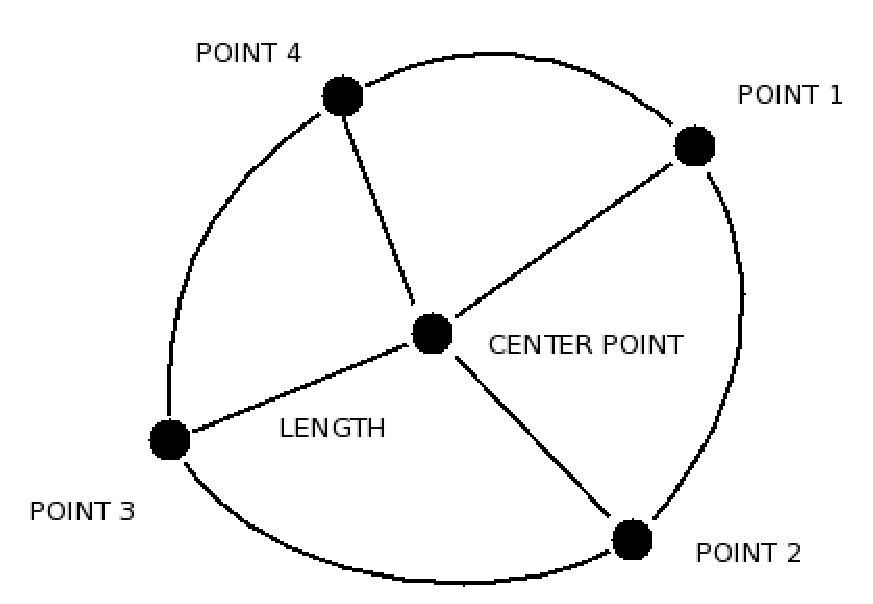
\includegraphics[scale=0.6]{p11.eps}
  \caption{Bunch construction scheme.}
  \label{bunch_example}
\end{center}
\end{figure}

A picture \ref{bunch_example} describes the construction scheme. The whole object 
is constructed around center point which also has maximal height.

\begin{verbatim}
{
  name = some_modificator_name
  type = MODIFICATOR_BUNCH

  /*
    [float]           height
    
    [float]           height_correction_center
    [float]           height_correction_left
    [float]           height_correction_top      
  */
  height = 1
  
  /*
    [float, interval] corner_curvature
  */
  corner_curvature = 0.4
    
  /*    
    [int, interval]   points
    [float, interval] lenght
  */
  points = 4
  lenght = 0.75  
    
  /*
    [float]           angle
    [int]             border
  */  
  angle = 0
  border = 0
}
\end{verbatim}
\subsubsection*{Bunch modificator properties}
\begin{itemize}
\item{\bf height} - maximal height of the emitted bunch (in the center point).
\item{\bf height\_correction\_center}
\item{\bf height\_correction\_left}
\item{\bf height\_correction\_top}
\item{\bf corner\_curvature} - curvature parameter in points. It's a number 
from \begin{math}<0,1>\end{math} range where 0 is totaly sharp and 1 is a circle.
\item{\bf points} - number of generated points (corners) of the bunch.
\item{\bf lenght} - a lenght between center point and the generated ones.
\item{\bf angle} - if the angle is set the angle between points is variated.
\item{\bf border}
\end{itemize}

\subsubsection*{Generated parameters}

\begin{center}
\begin{tabular}{|l||l|}
\hline
  Parameter & Meaning \\
\hline
\hline
  0 & pixel height \\
\hline  
\end{tabular}
\end{center}

\newpage
\subsection{Mask modificator}

\begin{verbatim}
{
  name = some_modificator_name
  type = MODIFICATOR_MASK

  /*
    Mask type:
  
    [enumerated type] mask_type
  
      MASK_BOOL
      MASK_COLOR
      MASK_HEIGHT
  */
  
  /*
    Mask sources:
  
    [string]          mask_bitmap
    
    [enumerated type] mask_source    
      TEXTURE
      GEOMETRY
      GENERATOR_MESH
      AUX
      MASK
      
    [string]          mask_source_name
    
    [vector]          mask_size
  */
}
\end{verbatim}
\subsubsection*{Mask modificator properties}
\begin{itemize}
\item{\bf mask\_type} - defines mask type
\begin{itemize}
\item{\bf MASK\_BOOL} - each pixel in mask is true/false values only.
\item{\bf MASK\_COLOR} - each pixel in mask contains RGB colors.
\item{\bf MASK\_HEIGHT} - each pixel in mask a float point number.
\end{itemize}
\item{\bf mask\_bitmap} - mask is loaded from image file.
\item{\bf mask\_source, mask\_source\_name} - mask is loaded from target. 
{\bf mask\_source} defines target type and {\bf mask\_source\_name} target name. 
If target name is unset, first target with requested type is used.
\item{\bf mask\_size} - mask is created as an empty mask with requested size.
\end{itemize}

\subsubsection*{Generated parameters}

None.

\newpage
\subsection{Light modificator}

Calculates light intensity for each pixel. Light values are written to target 
unless a slave modifiator is defined. If there is a slave modifiator defined, the
light modificator does not emit any pixels to target but passes light intensity as 
a parameter to slave modificator.

\begin{verbatim}
{
  name = some_modificator_name
  type = MODIFICATOR_LIGHT

  /*      
    [bool]    planar
      
    [vector]  light_position
      
    [float]   angle_min
    [float]   angle_scale
      
    [float]   specular_shine
      
    [color]   color_ambient
      
    [bool]    color_diffuse_active
    [color]   color_diffuse
      
    [bool]    color_specular_active
    [color]   color_specular
  */
  planar = 1
  light_position = (0,1,0)
  
  angle_min = 0
  angle_scale = 1
  
  color_ambient = (0,0,0,0)
  
  color_diffuse_active = 1
  color_diffuse = (1,1,1,1)
  
  color_specular_active = 0
  color_specular = (1,1,1,1)
  specular_shine = 1
}
\end{verbatim}
\subsubsection*{Mask modificator properties}
\begin{itemize}
\item{\bf planar} - Is the light planar or spot?
\item{\bf light\_position} - It's defined relative to target surface. 
\begin{math}<-1,y,-1>\end{math} means upper left corner of target surface and \begin{math}<1,y,1>\end{math} lower right
corner of target surface. The y value defines light height and it's from \begin{math}<0,1>\end{math} range, 
which is translated to \begin{math}<0,texture\_height>\end{math}.
\item{\bf angle\_min, angle\_scale} - An angle between surface normal vector and light vector
is modidified as:
\[
angle\_final = angle\_min + angle\_calculated * angle\_scale
\]
\item{\bf specular\_shine} - \begin{math}<0,1>\end{math} shine range.
\end{itemize}
Standard components of phong illumination model. A final light and final pixel color is calculated as:
\[
diffuse\_light = color\_ambient + (1 - angle\_final) * color\_diffuse
\]
\[
specular\_light = (1 - \frac{angle\_final}{specular\_shine}) * color\_specular
\]
\[
pixel\_color = pixel\_color * diffuse\_light + specular\_light
\]
\begin{itemize}
\item{\bf color\_diffuse\_active} - enables diffuse light component.
\item{\bf color\_specular\_active} - enables specular light component.
\item{\bf color\_ambient}
\item{\bf color\_diffuse}
\item{\bf color\_specular}
\end{itemize}

\subsubsection*{Generated parameters}

\begin{center}
\begin{tabular}{|l||l|}
\hline
  Parameter & Meaning \\
\hline  
\hline  
  0 & pixel light intensity \\
\hline
\end{tabular}
\end{center}

\newpage
\subsection{Target modificator}

Target modificator reads pixels from defined target (target\_name) and
puts it on parameter stack as parameters. It can be used by simple pixel modificator 
to write the data to another target.

\begin{verbatim}
{
  name = some_modificator_name
  type = MODIFICATOR_TARGET

  /*      
    [string]  target_name
  */
}
\end{verbatim}
\subsubsection*{Target modificator properties}
\begin{itemize}
\item{\bf target\_name} - source target name
\end{itemize}

\subsubsection*{Generated parameters}

\begin{center}
\begin{tabular}{|l||l|}
\hline
  Parameter & Meaning \\
\hline  
\hline  
  0 & pixel color, red component \\
  1 & pixel color, green component \\
  2 & pixel color, blue component \\
  3 & pixel color, alpha component \\
  4 & pixel color, height component \\
  5 & pixel normal vector, x component \\
  6 & pixel normal vector, y component \\
  7 & pixel normal vector, z component \\
\hline
\end{tabular}
\end{center}

\newpage
\subsection{Filter modificator}

Filter modificator can directly filter given target surface. 
It does not use any slave modificator because it writes data directly
to target surface.

\begin{verbatim}
{
  name = some_modificator_name
  type = MODIFICATOR_FILTER

  /*      
    [enumerated]  filter_target
      HEIGHT
      COLOR
      
    [enumerated]  filter_type
      INTERPOLATE
      BLUR
      
    [int]         filter_strength
  */
  filter_target = HEIGHT
  filter_type = INTERPOLATE
  filter_strength = 1  
}
\end{verbatim}
\subsubsection*{Filter modificator properties}
\begin{itemize}
\item{\bf filter\_target} - which component of target surface is filtered
\item{\bf filter\_type} - filter type
\item{\bf filter\_strength} - number of filter cycles
\end{itemize}

\subsubsection*{Generated parameters}
None

\subsection{Bitmap modificator}
TODO

\subsection{Generator modificator}
TODO

\end{document}
